\section*{Problem 2 Statement}

A ball is thrown horizontally from a height of 20 m and hits the ground with a speed that is three
times its initial speed. What is the initial speed? Assume that there is no air drag and therefore
acceleration in the horizontal direction is zero 

\bigbreak Given:
\begin{itemize}
    \item $\vec{v_0} = \frac{\vec{v}_{final}}{3}$
    \item $y_0$ = 20m
    \item $|v_{0y}| = 0, |v_{ox}| \neq 0$
\end{itemize}

Find:
\begin{itemize}
    \item $|\vec{v}_{init}|$
\end{itemize}

\section*{Solution}
\subsubsection*{Vertical speed}

A ball was thrown from the height $h = 20m$. Initial vertical speed was zero.
We can find final vertical speed as we know vertical acceleration $g = 9.81m/s^2$

$$ S_y = y_0 + v_{y0} \cdot t + a_y \cdot \frac{t^2}{2}$$

Now substitute data we have.

$$ 0 = 20m + 0m/s - 9.81m/s^2 \cdot \frac{t^2}{2}$$

Solving for $t$:

$$t = \sqrt{\frac{20m * 2}{9.81m/s^2}} \approx 2s$$

Now we can find $v_{yfinal}$ as we know time the ball travelled:

$$ g = \frac{v_{yfinal} - 0}{t}$$

Solving for $v_{yfinal}$:

$$v_{yfinal} = g * t = 9.81m/s^2 * 2s = 19,62m/s$$

\subsubsection*{Initial speed}
Let's proceed knowing $\vec{v_0} = \frac{\vec{v}_{final}}{3}$:

$$ \sqrt{v_{0x}^2 + v_{0y}^2} = \frac{\sqrt{v_{xfinal}^2 + v_{yfinal}^2}}{3} $$

$$ \sqrt{v_{0x}^2 + 0} = \frac{\sqrt{v_{xfinal}^2 + (19.62m/s)^2}}{3} $$

There was no horizontal acceleration. This means $v_{0x} = v_{xfinal}$.
\\ Substitute and find initial speed.

$$v_{0x} = \sqrt{\frac{v_{0x}^2 + (19.62m/s)^2}{3}}$$

$$9 \cdot v_{0x}^2 = v_{0x}^2 + 384.94(m/s)^2$$

$$v_{0x} = \sqrt{\frac{384.94(m/s)^2}{8}} $$

$$v_{0x} \approx 6.93m/s $$

$v_{0x}$ is actually the initial speed as no vertical speed existed.

$$|\Vec{v}_{init}| \approx \boxed{6.93m/s}$$

\hfill \newpage
\begin{figure}{h!}
    \centering
    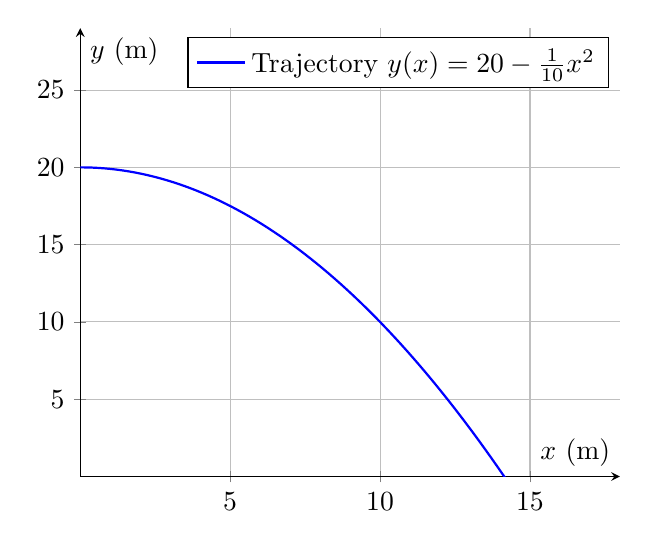
\begin{tikzpicture}
        \begin{axis}[
            xlabel={$x$ (m)},
            ylabel={$y$ (m)},
            xmin=0, xmax=18,
            ymin=0, ymax=29,
            axis x line=middle,
            axis y line=middle,
            grid=major,
            samples=100,
            domain=0:20,
        ]

        % Plot the trajectory y(x)
        \addplot[
            blue,
            thick
        ] {20 - (1 / 10) * x ^ 2};
        \addlegendentry{Trajectory $y(x) = 20 - \frac{1}{10}x^2$}
        \end{axis}
    \end{tikzpicture}
    \caption{Just found graph for fun}
    \label{fig:graphforfun}
\end{figure}


\vfill \subsection*{ANSWER}
\begin{itemize}
    \item 6.93m/s
\end{itemize}
